\documentclass{standalone}
\usepackage{tikz}
\begin{document}
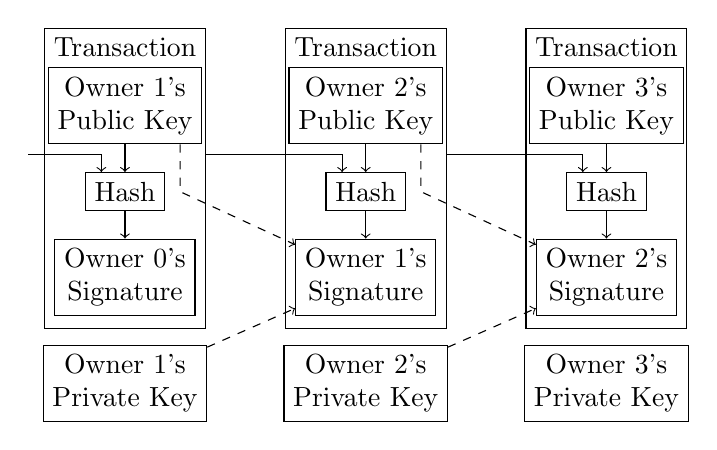
\begin{tikzpicture}
	\begin{scope}[every node/.append style={draw, text depth = 9.5em, anchor = west}]
		\node (trans1) {Transaction};
		\node (trans2) at ([xshift = 1cm] trans1.east){Transaction};
		\node (trans3) at ([xshift = 1cm] trans2.east){Transaction};
	\end{scope}

	\begin{scope}[every node/.append style={draw, align=center, anchor=north}]
		\node (pub1) at ([yshift=-5mm] trans1.north) {Owner 1's\\Public Key};%
		\node (hash1) at ([yshift = -1em] pub1.south) {Hash};%
		\node (sig0) at ([yshift=-1em] hash1.south) {Owner 0's\\Signature};%

		\node (pub2) at ([yshift=-5mm] trans2.north) {Owner 2's\\Public Key};%
		\node (hash2) at ([yshift = -1em] pub2.south) {Hash};%
		\node (sig1) at ([yshift=-1em] hash2.south) {Owner 1's\\Signature};%

		\node (pub3) at ([yshift=-5mm] trans3.north) {Owner 3's\\Public Key};%
		\node (hash3) at ([yshift = -1em] pub3.south) {Hash};%
		\node (sig2) at ([yshift=-1em] hash3.south) {Owner 2's\\Signature};
	\end{scope}

	\begin{scope}[every node/.append style={draw, align=center, anchor=north}]
		\node (priv1) at ([yshift=-2mm] trans1.south) {Owner 1's\\Private Key};
		\node (priv2) at ([yshift=-2mm] trans2.south) {Owner 2's\\Private Key};
		\node (priv3) at ([yshift=-2mm] trans3.south) {Owner 3's\\Private Key};
	\end{scope}

	\begin{scope}[->]
		\draw (pub1) -- (hash1);
		\draw (pub2) -- (hash2);
		\draw (pub3) -- (hash3);

		\draw (hash1) -- (sig0);
		\draw (hash2) -- (sig1);
		\draw (hash3) -- (sig2);

		\draw ([yshift = 3mm, xshift = -2mm] trans1.west) -| ([xshift = -3mm] hash1.north);
		\draw ([yshift = 3mm] trans1.east) -| ([xshift = -3mm] hash2.north);
		\draw ([yshift = 3mm] trans2.east) -| ([xshift = -3mm] hash3.north);
	\end{scope}

	\begin{scope}[->, dashed]
		\draw ([xshift=7mm] pub1.south) -- +(down:6mm) -- (sig1);
		\draw ([xshift=7mm] pub2.south) -- +(down:6mm) -- (sig2);

		\draw (priv1) -- (sig1);
		\draw (priv2) -- (sig2);
	\end{scope}
\end{tikzpicture}
\end{document}
